\documentclass[tikz, border=1pt]{standalone}
\pdfoutput=1 % if your are submitting a pdflatex (i.e. if you have
             % images in pdf, png or jpg format)

\usepackage{graphicx}

% Use the tikz package
\usepackage{tikz}
\usetikzlibrary{decorations}


\begin{document}

        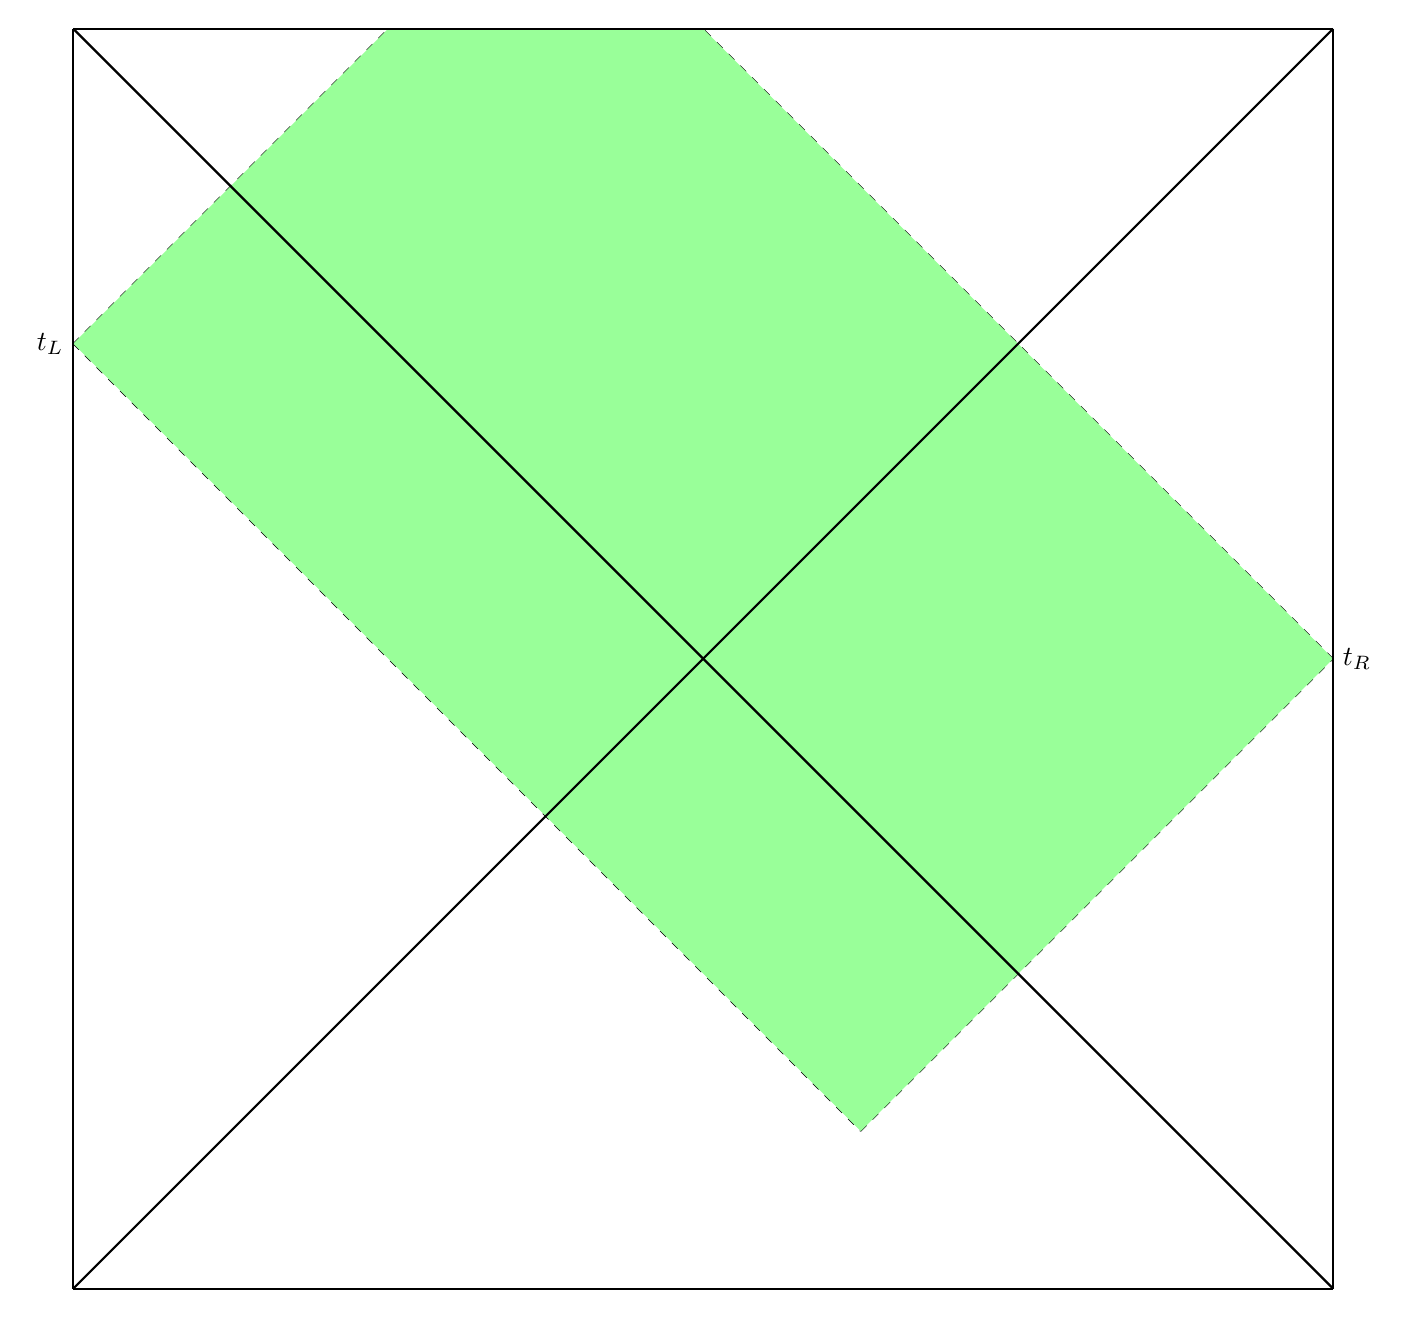
\begin{tikzpicture}[scale=4]
        
        % WdW boundaries
        \draw[dashed] (0,3)--(1,4); 
        \draw[dashed] (0,3)--(2.5,.5); 
        \draw[dashed] (2.5,.5)--(4,2);
        \draw[dashed] (4,2)--(2,4);
        \fill[green!40!white] (2,4)--(4,2)--(2.5,.5)--(0,3)--(1,4)--(2,4) ;
        
        %axes
        \draw[thick] (0,0)--(4,0);
        \draw[thick] (4,0) --(4,4);
        \draw[thick] (4,4)--(0,4);
        \draw[thick] (0,4)--(0,0);
        \draw[thick] (0,0) --(4,4);
        \draw[thick] (0,4)--(4,0);
        
        %labels
        \draw (0,3) node[left]{$t_L$};
        \draw (4,2) node[right]{$t_R$};
        %\draw (.75,2.1) node[right, rotate=-45]{$(v=v_L)$};
        %\draw (.65,3.5) node[right, rotate=45]{$(u=u_L)$};
        \end{tikzpicture}

\end{document}
